\section{Zielsetzung}
\label{sec:Zielsetzung}
Die effektive Masse beschreibt in der Festkörperphysik die scheinbare Masse von Teilchen in einem Kristall. In diesem Versuch wird die effektive Masse der Leitungselektronen von
n-dotiertem Galliumarsenid (n-GaAs) mithife des Effekts der Faradayrotation bestimmt. Der Faraday-Effekt bezeichnet die Drehung der Polarisationsebene von linear polarisiertem Licht
beim Durchgang durch ein Medium in einem Magnetfeld.

\section{Theorie}
\label{sec:Theorie}
\subsection{Bandstruktur}
\label{subsec:Bandstruktur}
Das Konzept der Bandstruktur ist elementarer Bestandteil der Festkörperphysik und beschreibt die Überlagerung diskreter Energieniveaus von Teilchen in einem Kristall. Das Valenzband
entspricht dem bei $T=\qty{0}{\kelvin}$ höchstem besetzten Energieband. Befinden sich freie Elektronen im darüber liegenden Leitungsband wird das Material leitend.
Es ergibt sich für verschiedene Materialien eine Struktur, die bestimmte Eigenschaften definiert. So ergibt es sich, dass Materialien mit einer großen Bandlücke zwischen 
Valenz- und Leitungsband einem Isolator entsprechen. Umgekehrt sind Materialien mit keiner Bandlücke Leiter. Ein schematisches Bild von Bandstrukturen ist in \autoref{fig:Bandstruktur}
zu sehen.

\begin{figure}
    \centering
    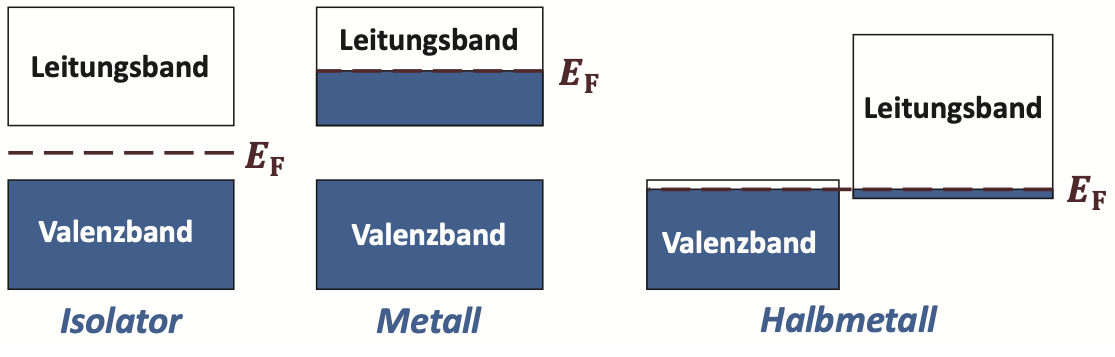
\includegraphics[width=\textwidth]{content/pics/Bandstruktur.png}
    \caption{Bandstruktur eines Isolators, Metalls und Halbmetalls. Hierbei bezeichnet $E_{\symup{F}}$ die Fermienergie \cite{GrossMarx2018}.}
    \label{fig:Bandstruktur}
\end{figure}

Materialien mit einer relativ kleinen Bandlücke von etwa $E_{\text{gap}}=\qtyrange{0}{6}{\electronvolt}$ weisen nochmal andere Eigenschaften auf und werden als Halbleiter
bezeichnet. Am absoluten Temperaturnullpunkt von $T=\qty{0}{\kelvin}$ ist ein Halbleiter nichtleitend, die Fermienergie liegt demnach in der Bandlücke. Für Raumtemperaturen liegt die
thermische Energie von Elektronen bei rund $E_{\text{therm.}}=\qty{26}{\milli\electronvolt}$. Hat ein Halbleiter eine Bandlücke in etwa diesem Energiebereich, treten Elektronen in das 
Leitungsband über und das Material wird leitend.

Die Bandlücke von dem in diesem Versuch verwendetem Galliumarsenid beträgt $E_{\text{gap, GaAs}} = \qty{1,42}{\electronvolt}$, somit befinden sich bei Raumtemperatur sehr wenig 
Elektronen im Leitungsband und die Leitfähigkeit ist entsprechend gering. Durch das Einbringen von Fremdatomen kann ein weiteres Energieniveau unterhalb des Leitungsbands geschaffen werden,
sodass sich zwischen diesem Band und dem Leitungsband eine deutlich kleinere Bandlücke ergibt. Das hier verwendete, n-dotierte Galliumarsenid hat eine Bandlücke in der Größenordnung der
thermischen Energie der Elektronen und wird somit leitend. 

\subsection{Effektive Masse}
\label{subsec:Effektive Masse}
Bewegt sich ein Teilchen in einem Kristall, so ist bei der Beschreibung der Bewegung das wirkende, periodische Gitterpotential zu berücksichtigen. Zur besseren Berechnung lässt
sich eine effektive Masse des Teilchens einführen, die ähnlich wie die reduzierte Masse zweier Körper in der Mechanik funktioniert.
Dazu wird die Energie des Leitungsbandes bis zur 2. Ordnung entwickelt
\begin{equation*}
    E(\mathbf{k}) = E(0) + \frac{1}{2}\sum_{\symup{i}=1}^{3}\left(\frac{\partial E^2}{\partial k_{\symup{i}^2}}|_{k=0}\right) k_{\symup{i}}^2 + ...
\end{equation*}

Der 2. Koeffizient lässt sich durch Umstellen der Gleichung des quantenmechanischen Oszillators 

\begin{equation*}
    E = \frac{\hbar k^2}{2m}
\end{equation*}

als effektive Masse

\begin{equation*}
    m_{\symup{i}}^{*}=\frac{\hbar^2}{\left(\frac{\partial E^2}{\partial k_{\symup{i}^2}}|_{k=0}\right)}
\end{equation*}

identifizieren. Aufgrund der Tatsache, dass das Gitterpotential für alle drei Raumrichtungen durchaus verschieden sein kann, handelt es sich bei der effektiven Masse um eine 
tensorielle Größe.


\subsection{Zirkulare Doppelbrechung}
\label{subsec:Zirkulare Doppelbrechung}
Doppelbrechung tritt in optisch aktiven Medien auf und beschreibt die Drehung der Polarisationsebene von linear polarisiertem Licht, was in \autoref{fig:Zirkulare Doppelbrechung} zu 
sehen ist. Linear polarisiertes Licht kann als Überlagerung von links und rechts polarisiertem Licht verstanden werden. Aufgrund der unterschiedlichen Phasengeschwindigkeiten kommt es
zum beschriebenen Effekt.

\begin{figure}
    \centering
    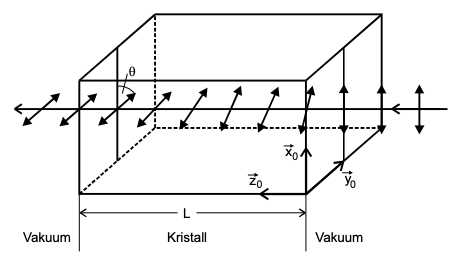
\includegraphics[width=0.8\textwidth]{content/pics/Zirkulare_Doppelbrechung.png}
    \caption{Illustration der zirkularen Doppelbrechung von linear polarisiertem Licht in einem Kristall \cite{V46_Anhang}.}
    \label{fig:Zirkulare Doppelbrechung}
\end{figure}

Der Rotationswinkel $\theta$ kann über die Brechungsindices für rechts und links polarisiertes Licht \eqref{eq:theta_rl_n} oder letzlich über die 
Suszeptibilität \eqref{eq:theta_rl_chi} ausgedrückt werden.

\begin{align}
    \theta &= \frac{L\omega}{2}\left(\frac{1}{n_{\symup{r}}}-\frac{1}{n_{\symup{l}}}\right) \label{eq:theta_rl_n} \\
    \theta &= \frac{L\omega}{2cn}\chi_{\text{xy}} \label{eq:theta_rl_chi} 
\end{align}

Hierbei bezeichnet $L$ die Strecke, die das Licht in dem optisch aktiven Medium zurücklegt.

\subsection{Faraday-Effekt}
\label{subsec:Faraday-Effekt}
In einem optisch inaktiven Medium kann unter normalen Umständen keine zirkulare Doppelbrechung beobachtet werden. Wird jedoch ein hinreichend starkes Magnetfeld parallel
zu der Ausbreitungsrichtung des Lichts angelegt, ist eine zirkulare Doppelbrechung zu beobachten. Dies wird als Faraday-Effekt oder Faradayrotation bezeichnet.

Die Suszeptibilität $\chi_\text{xy}$ ist von dem angelegten Magnetfeld abhängig
\begin{equation}
    \chi_\text{xy} = \frac{Ne^3\omega B}{\varepsilon_0\left(\left(-m\omega^2+K\right)^2-\left(e\omega B\right)^2\right)}.
    \label{eq:Suszeptibilität_Faraday}
\end{equation}

Wird für die Suszeptibilität in \eqref{eq:theta_rl_chi} \autoref{eq:Suszeptibilität_Faraday} eingesetzt, folgt
\begin{equation}
    \theta = \frac{e^3\omega^2 NBL} {2\varepsilon_0 cm^2\left(\left(\omega_0^2-\omega^2\right)^2-\left(\omega \cdot \omega_\text{c}\right)^2\right)n}.
    \label{eq:theta_fast_umgeformt}
\end{equation}
Hierbei wird $\omega_0 = \sqrt{\frac{K}{m}}$ als Resonanzfrequenz und $\omega_\text{c} = \frac{eB}{m}$ als Zyklotronfrequenz eingeführt. Dadurch, dass $\omega << \omega_0$ gilt
und durch Definieren von $\theta_\text{frei} = \frac{\theta}{L}$ als Faradayrotation pro Einheitslänge wird \autoref{eq:theta_fast_umgeformt} zu

\begin{equation}
    \label{eqn:theta_l2}
    \theta_\text{frei} = \frac{e^3 N B}{8\symup{\pi}^2 \varepsilon_0 c^3 (m^*)^2 n} \cdot \lambda^2.
\end{equation}
